% Official ICMLDE 2026 Procedia Computer Science template (Template_PROCS_ICMLDE_2026.zip):
% elsarticle.cls + ecrc.sty used unmodified; only content packages are added below.
\documentclass[3p,times,procedia]{elsarticle}
\flushbottom
\usepackage{ecrc}
\usepackage{amssymb,amsmath,booktabs,tabularx,array,longtable}
\usepackage{placeins}
\usepackage{tikz}
\usetikzlibrary{arrows.meta,positioning}
\usepackage{xr}
\usepackage{xurl}
\usepackage[bookmarks=false]{hyperref}
\hypersetup{colorlinks,linkcolor=blue,citecolor=blue,urlcolor=blue}
\volume{00}
\firstpage{1}
\journalname{Procedia Computer Science}
\runauth{Tushar Teotia et al.}
\jid{procs}
\newcommand{\code}[1]{\texttt{#1}}
\newcommand{\na}{\textnormal{n.a.}}
\setlength{\emergencystretch}{1em}

\begin{document}
\begin{frontmatter}
\dochead{5th International Conference on Machine Learning and Data Engineering}
\title{Oasis: A Mutation Testing Framework for Evaluating the Semantic Quality of Infrastructure-as-Code Test Suites}
\author[a]{Tushar Teotia}
\author[a]{Shiven Goomer}
\author[a]{Yash Vardhan Rawat}
\author[a]{Minakshi Tomer\corref{cor1}}
\author[a]{Manoj Kumar Malik}
\address[a]{Department of Information Technology, Maharaja Surajmal Institute of Technology, Janakpuri, New Delhi 110058, India}
\begin{abstract}
Infrastructure-as-Code (IaC) test suites may pass despite there being faults in their tested configuration. We introduce Oasis, a
mutation testing framework using minor changes to HCL within native Terraform and OpenTofu test suites. Oasis checks whether a
mutated variable default can reach the chosen tests, differentiates between assertion and runtime errors,
and ensures that source files are restored afterwards. We assessed a fixed catalog with 16 operators against a filtered sample of 62
repositories. Oasis generated 1,533 mutants, and 1,288 of them, from 47 repositories, were scored, resulting in 115 assertion killed
mutants, 76 runtime error killed mutants and 1,097 survivor mutants. This gives 8.9\% assertion kill rate and 14.8\% overall kill
rate. A further 245 mutants were excluded, generally as context specific no-ops. Generic mutators producing Boolean inversions resulted
in 89.1\% of scored mutants. Through a separate study of 123 fixed mutants we saw that enhancing existing tests raised the
number of mutants caught by assertions from 39 to 73. The median time taken to test a mutant was 11.6s. These results provide
an indication of how sensitive tests are given a set of fixtures/mocks but do not give any indication of the actual fault rates or
security levels in live clouds.



\end{abstract}
\begin{keyword}
Infrastructure-as-Code \sep Terraform \sep OpenTofu \sep Mutation Testing \sep Test Oracles \sep Reproducibility
\end{keyword}
\cortext[cor1]{Corresponding author.}
\end{frontmatter}
\email{tomer.minakshi@gmail.com}

\section{Introduction}\label{sec:introduction}
Infrastructure-as-Code allows infrastructure to be version controlled. However, syntactically correct configurations can still disable encryption, leave network access open or remove capacity. Terraform and OpenTofu now have built-in testing frameworks that allow assertions to be made on plan or apply operations, often using mocked providers
~\cite{terraformtests,tofutests,mocks}. However, a passing test suite may only confirm that the configuration executes successfully, rather than verifying that it enforces the intended properties.


Mutation testing can be used to provide this information directly, by introducing changes to the program and seeing if they are detected by the tests~\cite{jia,papadakis}. However there are several issues when applying mutation testing to native IaC suites. Firstly, if the test chosen provides a value then changing the default of a variable will have no impact; increasing the number of survivors in naive mutation. Secondly, tests that fail anyway should not be considered as kills. Finally mutants that are rejected due to a runtime error are different to mutants that are detected by an assertion checking a requirement.

Oasis addresses these issues by (i) introducing a mutation-testing pipeline for native test-suites with multiple mutation operators and baseline, validity and source recovery gates. We also include a conservative check to determine that a mutated default can reach the chosen tests. (ii) We perform a versioned multi-repository experiment which provides useful output including blocked and excluded work. (iii) We conduct a matched test-strengthening study and a separate historical comparison with a policy scanner. Ribeiro and Neves~\cite{ribeiro} recently developed mutation operators for Terraform from corrective commits, however they only demonstrate their operators on one reference project. Our work is not the first Terraform mutation tool, but we bring a systematic approach to evaluating how existing native suites perform on mutation. We show few changes to the configuration are detected by assertion (8.9\%), 40\% of kills come from runtime errors and using mutation feedback can almost double the number of assertion detections when improving tests.

We address four research questions. \textbf{RQ1}: Which repository scopes produce usable outcomes, and which are blocked? \textbf{RQ2}: How do operators and operator families perform? \textbf{RQ3}: Can test strengthening change detections on the same fixed mutants? \textbf{RQ4}: What does mutation execution cost, and how do native outcomes relate to policy-scanner findings? Section~\ref{sec:related} reviews related work, Sections~\ref{sec:design} and~\ref{sec:method} describe the design and method, Section~\ref{sec:results} reports results, and Sections~\ref{sec:implications}--\ref{sec:conclusion} discuss implications, threats to validity and conclusions.

\section{Background and related work}\label{sec:related}
\textbf{IaC defects.} Rahman et al. correlate script quality with defects in IaC code \cite{rahman}, catalogue security smells~\cite{seven}, and define the ``Gang of Eight'' IaC defect taxonomy: conditional, configuration data, dependency, documentation, idempotency, security, service and syntax defects~\cite{gangofeight}. Drosos et al.\ study faults in IaC ecosystems such as Ansible, Puppet and Chef~\cite{drosos}, and Verdet et al.\ measure security-policy adoption in Terraform projects~\cite{verdet}. Most similar to our work, Ribeiro and Neves clustered 6,749 corrective commits from 54 Terraform repositories into defect categories. They identified nine mutation operator families and developed a prototype tool, Terramutate, to demonstrate this~\cite{ribeiro}. They also identified systematic evaluation and whether tests that kill mutants can detect real faults as areas for future work. Oasis was developed independently and in parallel to this work. This work was published in July 2026 while Oasis was being developed. Both studies therefore arrived at related operator families, although they approached the problem from different starting points.


\textbf{IaC testing and analysis.} ProTI is a tool that uses test generation, mocking and pluggable oracles to test Pulumi programs~\cite{proti}. EMIaC uses metamorphic testing on IaC engines~\cite{emiac}. GLITCH statically identifies IaC smells~\cite{glitch,glitchdemo}. Testing itself remains uncommon: Hasan et al.\ catalogue the testing practices used for IaC~\cite{hasan}. The authors of ProTI found less than 1\% of public Pulumi and CDK programs on GitHub had tests in August 2022~\cite{proti}. This motivates tools that can help determine if existing tests are effective. Table~\ref{tab:capabilities} shows how these methods differ from Oasis, which alters configuration values and watches how a native test suite behaves.

\begin{table}[ht]
\caption{Testing targets of related approaches (a comparison of purpose, not of speed or accuracy).}\label{tab:capabilities}
\small\begin{tabularx}{\linewidth}{@{}p{2.1cm}XX@{}}\toprule
Approach & Object and oracle & Relationship to Oasis\\\midrule
Terramutate~\cite{ribeiro} & Terraform operators derived from corrective-commit themes; one reference project & Oasis evaluates native suites across many repositories; neither establishes coupling to real faults.\\
ProTI~\cite{proti} & Pulumi TypeScript programs; generated configurations and property oracles & Generates tests rather than assessing an existing HCL suite.\\
EMIaC~\cite{emiac} & IaC engines; semantics-preserving transformations & Targets engine bugs, not test-suite sensitivity.\\
Oasis & Native Terraform/OpenTofu suites; existing assertions & Mutates configuration values and attributes assertion and runtime outcomes.\\\bottomrule
\end{tabularx}\end{table}

\textbf{Mutation testing.} Surveys address the design of mutation operators, costs, and equivalent mutants~\cite{jia,papadakis,madeyski}. In application code, mutant detection correlates with real-fault detection~\cite{just}. However, much of this correlation can be attributed to test suite size~\cite{papadakis2018}; coverage is also a poor measure of effectiveness~\cite{coverage}. Mutation testing has also been applied on an industrial scale~\cite{practices,scale} and studied among practitioners~\cite{sanchez}. Mutation scores reported in these studies are not directly comparable with ours because the operators, fault pools and filtering differ, so we do not rank Oasis against them or derive an adequacy threshold.

\section{Oasis design}\label{sec:design}
\subsection{Execution pipeline}
Oasis has been written in Python. It identifies valid literals from local HCL files and logs the file name, offset,
original value and replaced value of each mutation. It applies one change at a time without reformatting the surrounding code.
A scope is a repository, module directory and chosen test directory. Modules pulled from the registry are run as
dependencies but will not be mutated. Two mutant cases will be created by applying the same change to two different
scopes.

For each scope, Oasis will setup dependencies, execute unchanged tests/validation, check the candidate's
input context, validate all mutants, execute native tests, classify the results and reset the source (Fig.~\ref{fig:pipeline}). If the baseline fails, no mutant is reported as a kill. Timeout, invalid mutants, unresolvable context and no-ops will be reported as excluded results. All results will have information on their source hash, operator, scope and command record.

\begin{figure}[ht]
\centering
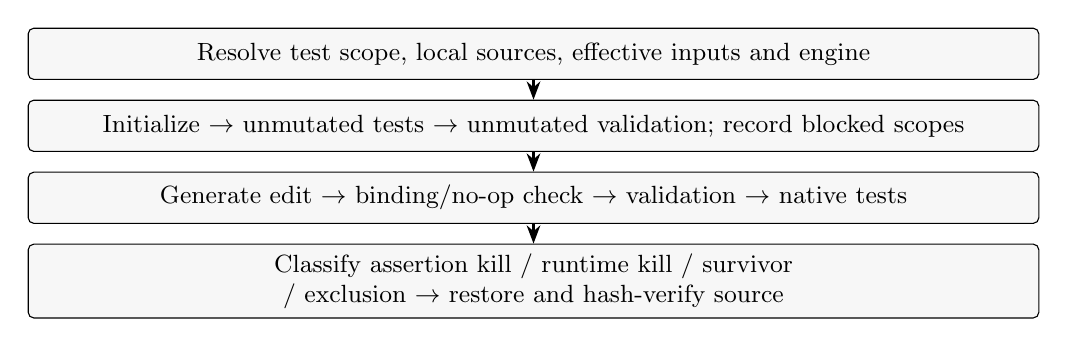
\begin{tikzpicture}[node distance=2.5mm,font=\small,b/.style={draw,rounded corners=2pt,align=center,minimum height=6.5mm,text width=12.6cm,fill=black!3},a/.style={-{Stealth},thick}]
\node[b] (a) {Resolve test scope, local sources, effective inputs and engine};
\node[b,below=of a] (b) {Initialize $\rightarrow$ unmutated tests $\rightarrow$ unmutated validation; record blocked scopes};
\node[b,below=of b] (c) {Generate edit $\rightarrow$ binding/no-op check $\rightarrow$ validation $\rightarrow$ native tests};
\node[b,below=of c] (d) {Classify assertion kill / runtime kill / survivor / exclusion $\rightarrow$ restore and hash-verify source};
\draw[a] (a)--(b);\draw[a] (b)--(c);\draw[a] (c)--(d);
\end{tikzpicture}
\caption{Native mutation pipeline.}\label{fig:pipeline}
\end{figure}

\subsection{Operator catalog and fault rationale}\label{sec:operators}
The initial investigation fixed framework version \code{0.3.0-research.1} (catalog~3: 16 operator identifiers, 22 hashed source files) before execution. Twelve operators from the original submission were carried forward (Table~\ref{tab:operators}). Four new operators have been introduced including Boolean MUT-CFG-001. This new operator focuses on module input arguments (M), and scalar variable defaults (V). It is worth noting that edits made by two operators are counted once within each scope, attributed to the more specific operator.


\begin{table}[ht]
\caption{Frozen catalog 3. Surfaces: R, resource or module body; V, variable default; L, local value; M, module input argument.}\label{tab:operators}
\small\begin{tabularx}{\linewidth}{@{}p{3.05cm}Xp{1.4cm}@{}}\toprule
Identifier(s) & Transformation & Surface\\\midrule
MUT-SEC-001 & S3 private ACL to public-read & R\\
MUT-SEC-002 & Storage encryption true to false & R\\
MUT-SEC-003 & Restrictive CIDR to 0.0.0.0/0 & R\\
MUT-SEC-004a--d & Disable one of four S3 public-access-block flags & R\\
MUT-RES-001 & Instance size to a larger class & R,V\\
MUT-RES-002 & Count/desired/minimum of at least two to one & R,V\\
MUT-RES-003 & Positive replica count to zero & R,V\\
MUT-TAG-001 & Environment tag production to development & R,V,L\\
MUT-TAG-002 & Delete a team/owner/cost\_center tag & R,L\\\midrule
MUT-CFG-001 (added) & Boolean literal inversion, including caller and default sites & R,V,L,M\\
MUT-RES-004 (added) & Positive capacity/count to zero & R,V\\
MUT-SEC-005 (added) & EC2 IMDS tokens required to optional & R,V\\
MUT-SEC-006 (added) & EFS/Redshift encryption true to false & R\\\bottomrule
\end{tabularx}\end{table}

\textbf{Relation to defect taxonomies.} All operators make literal edits, meaning, in terms of the Gang of Eight taxonomy~\cite{gangofeight} they represent configuration data defects. Access and encryption operators also represent security defects. Oasis does not model conditional, dependency, documentation, idempotency, service or syntax defects. Table~\ref{tab:mapping} provides a summary of how the taxonomy aligns to the Terraform specific taxonomy of Ribeiro and Neves~\cite{ribeiro}. Oasis does not implement their version constraint, suppression comment, IAM policy, provider or module declaration families. Due to the Ribeiro and Neves taxonomy being based on commit message analysis (rather than analysing at patch level) this shows our operators are plausible but do not confirm they replicate real faults. A detailed breakdown of the mappings for each identifier can be found in the supplement (Tables S3 and S4) alongside documented reasoning for each edit.

\begin{table}[ht]
\caption{Correspondence of Oasis operator groups with the Gang of Eight categories~\cite{gangofeight} and the variants of Ribeiro and Neves~\cite{ribeiro}. ``Direct'': same stated edit; ``partial'': related but different edit; ``generic'': only their broad attribute change applies. The \code{MUT-} prefix is omitted.}\label{tab:mapping}
\small\begin{tabularx}{\linewidth}{@{}>{\raggedright\arraybackslash}p{4.2cm}>{\raggedright\arraybackslash}p{3.3cm}>{\raggedright\arraybackslash}X@{}}\toprule
Oasis operators & Gang of Eight & Ribeiro and Neves\\\midrule
Boolean inversion (\code{MUT-CFG-001}, \code{SEC-002}, \code{SEC-004a--d}, \code{SEC-006}) & Configuration data; security for access/encryption flags & \code{PAR\_BOOL}, \code{VDR\_DEF} for defaults (direct)\\
CIDR widening (\code{SEC-003}) & Configuration data; security & \code{RCR\_SG\_OPEN} (direct)\\
Tag deletion / change (\code{TAG-002}, \code{TAG-001}) & Configuration data & \code{RCR\_TAG\_DEL} (direct); \code{RCR\_ATTR} (generic)\\
Capacity and replicas (\code{RES-002}--\code{004}) & Configuration data & \code{PAR\_NUM} (partial: to zero or one, not $\pm1$)\\
ACL, instance class, IMDS (\code{SEC-001}, \code{RES-001}, \code{SEC-005}) & Configuration data; security for ACL/IMDS & \code{RCR\_ATTR} (generic)\\\midrule
Not modelled by Oasis & Conditional, dependency, documentation, idempotency, service, syntax & Version constraints, suppression comments, IAM policy, provider and module declarations\\\bottomrule
\end{tabularx}\end{table}

\subsection{Context-specific no-ops}\label{sec:equivalence}
Oasis does not solve generalised mutant equivalence but removes a subset of mutants where a variable default has been mutated but cannot be seen by the chosen tests as all callers provide their own value. For each mutated default, the resolver looks through the chosen test files and the local callers in the repository. Each path is labelled as being active (the default may have an effect such as an argument being omitted or a non-nullable input receiving null), shadowed (a literal has independently overridden the value) or unresolved (an expression, unsupported format or external input prevents a decision). If any paths are active then the mutant will be tested. If all paths are shadowed then the mutant will be excluded as the mutation would have no effect. Otherwise, if any paths are unresolved then they will be excluded. Root tests are treated more strictly than nested calls. The analysis is engine aware. If a scope is run on OpenTofu then the file semantics apply. This means that any .tofu file will override a .tf file of the same name and any .tofutest.hcl file will override a .tftest.hcl file~\cite{tofufiles}. Therefore defaults and test inputs will be resolved from the code that OpenTofu runs. The full decision table can be found in the supplement (Table S2). Survivors will never be removed due to the scanner being silent or a mock hiding the value. Mutants not known to be equivalent remain in the denominator.

\section{Empirical method}\label{sec:method}
\subsection{Repository selection}\label{sec:selection}
There were 95 unique upstream repositories included in the study design (23 original study repositories in their previously adapted form, 37 new additions and 35 static filter passed repositories). A number of repositories were identified from searching available public Terraform projects, and then manually filtered to ensure they had some native testing, could be run with mocks and had at least one site in local code for a catalog operator. They were also not filtered on kill rates, although previous results were visible. The sample therefore is a technically screened convenience sample, not a representative population of Terraform users.
A time based cut-off was applied. Any repositories currently being run were allowed to complete, however any repositories waiting to retry or that had not begun were not. Smaller workloads were prioritised. There were a total of 62 repository attempts completed at the reporting date (9th November 2026). Three failed at the preparation stage, one was still running and so was excluded, and finally 29 had not begun. All statuses have been retained.


\subsection{Execution and source policy}\label{sec:adaptation}
Tests were run natively on Terraform 1.16.7 or OpenTofu 1.12.3 (four repositories) with timeouts
applied for setup (900s), test-running (600s) and validation (600s). All suitable mutants within a scope with a
passing baseline were run, no upper limit on mutants. Provider versions were locked and hashes verified. No
cloud credentials and no real provisioning occurred. No assertions, mocks or test values were modified during
the catalog 3 campaign. However, the 23 original study repositories still have previous modifications to their
setup. This includes synthetic inputs, mocks, repair of dependencies, some assertion repairs and removal of assertions whose conditions were constant. Complete records of these changes are not available for every repository, but the known modifications are documented in the supplement
 (Tables S9 and S10).

\subsection{Metrics}\label{sec:metrics}
Let $A$ be assertion kills, $E$ runtime-error kills and $S$ survivors among valid mutants in scopes with a passing baseline:
\begin{equation}
N=A+E+S,\qquad D_A=A/N,\qquad MS=(A+E)/N.\label{eq:score}
\end{equation}
$D_A$ measures assertion sensitivity; $MS$ also credits runtime rejection. Timeouts, invalid mutants, no-ops and unresolved contexts are excluded from both. Repositories with $N=0$ receive no score rather than zero. The twelve retained and four added operators run on the same catalog~3 engine, so comparing them is a within-version split, not a rerun of the original study.

\subsection{Matched strengthening, scanner and cost protocols}\label{sec:paired}
\textbf{Historical study.} The original catalog~2 study covered 23 repositories: 299 generated mutants, of which 276 were scored (47 assertion kills, 2 runtime kills, 227 survivors). Its results are reported separately and never pooled with catalog~3.

\textbf{Matched strengthening (RQ3).} We froze 123 mutants across 40 modules in 8 repositories. These were tested with
original tests and enhanced tests. Enhanced tests involved adding 63 assertions and 37 positive control runs.
No changes were made to source code, existing runs or mocks. As new inputs are covered by the added runs, the gain cannot be attributed to the added assertions alone. Cases were divided into 95 development and 28 transfer cases (from two different
repositories). While proposals were locked before running transfer cases, the researchers had seen the results from the pilot study so it is not a blind hold out.

\textbf{Scanner comparison (RQ4).} On the 23 historical snapshots, tfsec~1.28.14~\cite{tfsec} scanned each unmutated and mutated module without downloading remote modules. A mutant counts as flagged only if a newly reported rule overlaps the mutated line; existing findings earn no credit. \textbf{Cost (RQ4).} We report per-command durations for initialization, baseline runs, mutant validation and mutant tests, including failures and timeouts. Sums overlap across workers and are not wall-clock time.

\section{Results}\label{sec:results}
\subsection{RQ1: completion and exclusions}\label{sec:completion}
A summary of the 95 repository plan is shown in Table~\ref{tab:overview}. Of the 192 completed scopes, 130 had a passing baseline whilst 62 were blocked. A total of 47 repositories generated scored mutants, with 39 having all selected baselines passing, and 8 having some blocked scopes. Fifteen completed repositories did not generate any scored mutants. The different groups of admissions have differing DA values: 7.9\% for the 11 scored repositories from the original study (N=507), 10.6\% for the 14 added later (N=379) and 8.7\% for the 22 reserves (N=402). These groups differ in source and sampling and are not matched.


\begin{table}[ht]
\caption{Disposition of the 95-repository plan at the 9 November 2026 snapshot.}\label{tab:overview}
\small\begin{tabularx}{\linewidth}{@{}Xr@{}}\toprule
Disposition & Count\\\midrule
Completed, scored mutants, all selected baselines pass & 39\\
Completed, scored mutants, some baselines blocked & 8\\
Completed, no scored mutants & 15\\
Preparation failed (retries cancelled) / still running (excluded) / not started & 3 / 1 / 29\\
Completed scopes: passing / blocked baseline & 130 / 62\\
Generated mutants: scored / excluded & 1,288 / 245\\\bottomrule
\end{tabularx}\end{table}

From a total of 1,533 mutants, only 1,288 mutants were scored. 245 mutants were excluded in total. 193 were excluded due to no-ops in specific contexts. 39 mutants were removed due to unresolvable contexts and 13 due to timeout. Mutants in blocked scopes were never generated, so their number is unknown. The LangChain repository illustrates this: the AWS and GCP scopes resulted in 233 mutants being scored. However, the Azure scope was unable to reach baseline. This was because of an error that occurred when downloading from the provider. We received an HTTP 504 error. Other reasons for blocked scopes were missing sources, errors during the initialisation of the providers, dependencies on external programs and tests conflicting with the source configuration.

\subsection{RQ2: operator outcomes}\label{sec:operatorresults}
Overall, the scored mutants included 115 assertion kills, 76 runtime error kills and 1,097 surviving mutants (DA = 8.9\%, MS = 14.8\%). Per repository, the mean combined kill rate was 33.5\% and the median 18.2\%. All operators used are shown in Table~\ref{tab:operatorresults}. As MUT-CFG-001 comprises 89.1\% (1,147) of the mutants, the overall figures are driven by the sensitivity of test cases to configuration flags. The security operators had a DA of 13.4\% (N=67). Resource operators had a DA of 4.2\% (N=72), and most of their kills (24 of 27) were runtime errors. The twelve retained operators had 77 scored mutants with a DA of 11.7\%. The four added operators had 1,211 mutants with a DA of 8.8\%. Overall there were 1,049 unique edits across all repositories. These represent scored mutants as opposed to actual defects within infrastructure. A breakdown by admission group, operator family and subfamily, along with further examples, can be found in the supplementary information (Tables S5--S8).

\begin{table}[ht]
\caption{Outcomes for all 16 operators. Gen.: generated; Excl.: excluded; $D_A=A/N$; $MS=(A+E)/N$; n.a.: no scored mutants.}\label{tab:operatorresults}
\small\begin{tabularx}{\linewidth}{@{}Xrrrrrrrr@{}}\toprule
Identifier & Gen. & $N$ & $A$ & $E$ & $S$ & Excl. & $D_A$ & $MS$\\\midrule
\code{MUT-CFG-001} & 1,363 & 1,147 & 102 & 51 & 994 & 216 & 8.9\% & 13.3\%\\
\code{MUT-RES-001} & 19 & 9 & 0 & 1 & 8 & 10 & 0.0\% & 11.1\%\\
\code{MUT-RES-002} & 8 & 4 & 0 & 0 & 4 & 4 & 0.0\% & 0.0\%\\
\code{MUT-RES-003} & 3 & 3 & 0 & 0 & 3 & 0 & 0.0\% & 0.0\%\\
\code{MUT-RES-004} & 67 & 56 & 3 & 23 & 30 & 11 & 5.4\% & 46.4\%\\
\code{MUT-SEC-001} & 1 & 1 & 0 & 0 & 1 & 0 & 0.0\% & 0.0\%\\
\code{MUT-SEC-002} & 4 & 4 & 1 & 0 & 3 & 0 & 25.0\% & 25.0\%\\
\code{MUT-SEC-003} & 2 & 2 & 0 & 0 & 2 & 0 & 0.0\% & 0.0\%\\
\code{MUT-SEC-004a} & 14 & 13 & 3 & 0 & 10 & 1 & 23.1\% & 23.1\%\\
\code{MUT-SEC-004b} & 14 & 13 & 2 & 0 & 11 & 1 & 15.4\% & 15.4\%\\
\code{MUT-SEC-004c} & 14 & 13 & 1 & 0 & 12 & 1 & 7.7\% & 7.7\%\\
\code{MUT-SEC-004d} & 14 & 13 & 1 & 0 & 12 & 1 & 7.7\% & 7.7\%\\
\code{MUT-SEC-005} & 7 & 7 & 1 & 0 & 6 & 0 & 14.3\% & 14.3\%\\
\code{MUT-SEC-006} & 1 & 1 & 0 & 0 & 1 & 0 & 0.0\% & 0.0\%\\
\code{MUT-TAG-001} & 2 & 2 & 1 & 1 & 0 & 0 & 50.0\% & 100.0\%\\
\code{MUT-TAG-002} & 0 & 0 & 0 & 0 & 0 & 0 & \na & \na\\\midrule
Total & 1,533 & 1,288 & 115 & 76 & 1,097 & 245 & 8.9\% & 14.8\%\\\bottomrule
\end{tabularx}\end{table}

\textbf{Worked example.}\label{sec:workedexample} In \code{equinor/terraform-azurerm-key-vault}, the variable \code{purge\_protection\_enabled} defaults to true (\path{variables.tf:32}) and is passed to \code{azurerm\_key\_vault.this}. The existing plan run \code{soft\_delete\_defaults} uses a mocked Azure provider and omits this input, so the default is active. Its assertion at line~26 checks \code{purge\_protection\_enabled == true}. Inverting the default to false produced a valid mutant that failed exactly this assertion: the unmutated suite passed 25 runs, the mutant 24 with one assertion failure. Purge protection prevents a deleted vault from being purged during its retention period~\cite{azurepurge}, so the test guards a meaningful contract. By contrast, inverting \code{enable\_key\_rotation} on \code{aws\_kms\_key.eks} in \code{ambicuity/terraform-aws-eks-ray} survived. A survivor shows only that the recorded inputs and mocks accepted the change; missing assertions, inactive code paths, mock behavior or genuine equivalence can all explain it.

\subsection{RQ3: test strengthening}\label{sec:pairedresults}
\begin{table}[ht]
\caption{Matched 123-mutant comparison; the same mutants are run against original and strengthened tests.}\label{tab:paired}
\small\begin{tabularx}{\linewidth}{@{}Xrrrr@{}}\toprule
Subset & Mutants & Original $A$ & Strengthened $A$ & New detections\\\midrule
Development & 95 & 34 & 56 & 22\\
Transfer (two repositories) & 28 & 5 & 17 & 12\\\midrule
Total & 123 & 39 & 73 & 34\\\bottomrule
\end{tabularx}\end{table}
The total number of assertion detections increased from 39/123 (31.7\%) to 73/123 (59.3\%). There were no losses (Table~\ref{tab:paired}). The number of survivors decreased from 82 to 48. The increases were mostly in S3 public access block mutants, with 32 of the 34 gains originating from there. All 12 transfer-related gains came from one repository (serverless-architecture-patterns). This demonstrates that we can use mutation feedback to find areas to improve; however, it does not establish whether these improvements would generalise beyond the evaluated cases.

\subsection{RQ4: cost and scanner comparison}\label{sec:costs}
\begin{table}[ht]
\caption{Native command durations in seconds, including failures and timeouts. Sums are command time, not wall-clock time.}\label{tab:costs}
\small\begin{tabularx}{\linewidth}{@{}Xrrrr@{}}\toprule
Phase & Commands & Sum & Median & P95\\\midrule
Initialization & 191 & 1,641.1 & 4.57 & 24.97\\
Unmutated test & 165 & 3,102.2 & 13.21 & 35.11\\
Unmutated validation & 131 & 571.1 & 3.06 & 14.17\\
Mutant validation & 1,301 & 8,426.9 & 5.57 & 14.17\\
Mutant test & 1,301 & 94,002.5 & 11.59 & 386.88\\\bottomrule
\end{tabularx}\end{table}
Table~\ref{tab:costs} shows that mutant tests account for most of the cost: 1,301 runs (1,288 scored + 13 timeouts) and 94,002 seconds of command duration. The median is 11.6 seconds, but 95th percentile is 387 seconds. This means that the speed of the baseline cannot be used to predict the cost of running a complete mutation run. This depends on the number of sites, failed paths and timeouts. The measurements are all made using one run with warm caches. We can make no claims about a saving in cost, or differences in engine performance.

\begin{table}[ht]
\caption{Historical catalog~2 mutants (276) by native outcome and tfsec result. ``New site rule'': a newly reported rule overlaps the mutated line.}\label{tab:scanner}
\small\begin{tabularx}{\linewidth}{@{}Xrrr@{}}\toprule
Scanner result & Assertion kill & Runtime kill & Survivor\\\midrule
New site rule & 38 & 0 & 88\\
No new site rule & 9 & 2 & 94\\
Scan unavailable & 0 & 0 & 45\\\midrule
Total & 47 & 2 & 227\\\bottomrule
\end{tabularx}\end{table}
For the scanner comparison (Table~\ref{tab:scanner}), 231 of the 276 historical mutants could be compared; the other 45 (from the GenAI and Psoxy repositories) failed because tfsec rejects newer HCL blocks such as \code{check} and \code{removed}. Of the 231, 126 triggered a new rule at the mutated line, including 88 that the native tests accepted; conversely, 9 assertion kills triggered no new rule. For example, setting \code{block\_public\_acls} to false in \code{aws-platform-starter} survived the native tests but triggered \code{aws-s3-block-public-acls}, whereas the same edit in \code{platform-design} was killed by an assertion without a new rule.

\textbf{Survivors and prior misconfiguration research.} The 88 flagged survivors are configurations that a policy scanner would warn about but the project's tests accept, which is consistent with Verdet et al.'s observation that security policies are unevenly adopted in Terraform projects~\cite{verdet}. The 9 unflagged assertion kills show the reverse: project tests can encode contracts that generic policies do not. Since the catalog 3 sample is dominated by Boolean inversions, we do not assume that the prevalence of security policies is reflected in our survivors, and we do not treat a lack of scanning evidence as evidence of equivalence.

\section{Discussion}\label{sec:implications}
\textbf{Naive mutation would misreport IaC suites.} If we omit the binding check, then 193 shadowed defaults would be counted as survivors, even though no chosen test can observe them. This lowers the assertion-detection rate to 7.8\% from 8.9\%. Furthermore, 76 of the 191 killed mutants (39.8\%) were killed by runtime errors rather than assertion failures. For resource operators, this figure increases to 24 out of 27. Therefore, considering a single score could give a misleading picture of how well the tests are checking for the desired property.

\textbf{Many suites are mainly smoke tests.} Out of the 47 repositories where scores were obtained, 18 had zero assertion kills, and 14 had zero kills. The three largest repositories provide the bulk of data for these results (741 out of 1,288 mutants scored, 57.5\% of total). This is why the pooled rate (14.8\%) and the per-repository median (18.2\%) are much lower than the per-repository mean (33.5\%). As such, results should be interpreted on a per repository level. Overall, Oasis is most useful when used as an indication of where unchecked settings are occurring in the system.

\textbf{Survivors are actionable.} With a total of 63 inserted assertions and 37 positive controls, 34 previously surviving mutants were detected by assertions with no changes to the infrastructure source code. Combined with the fact that 88 survivors in the scanner comparison triggered policy-scanner rules, it seems sensible to identify which survivors affect security-sensitive areas and add targeted assertions where appropriate. The cost data suggests that we should run this type of analysis on a subset of modules or in batch jobs, as the median is 11.6 s per mutant but there is a long tail.

\section{Threats to validity}\label{sec:threats}\label{sec:discussion}
\textbf{Construct validity.} Oasis measures sensitivity to a bounded set of literal edits. The operator mapping in Section~\ref{sec:operators} is analytical; it is not patch-level validation or a measurement of coupling to real faults, and Boolean inversion dominates the sample. Runtime rejection is not an assertion oracle, and the no-op check does not solve general equivalence. \textbf{Internal validity.} Fixtures, mocks, earlier preparation changes (including some assertion repairs in the 23 original repositories), dependency resolution and timeouts affect outcomes; a passing mocked baseline does not certify a live deployment. \textbf{External validity.} The sample is a screened convenience sample of public, mock-compatible projects closed by a deadline after some outcomes were visible. Mutants cluster by repository and repeat edits across scopes, so pooled rates are descriptive and no significance tests are reported. The strengthening study had pilot exposure and investigator-written treatments. \textbf{Comparison validity.} Line-based scanner matching can miss indirect findings or match unrelated rules, and scanner and test inputs differ, so we make no precision or recall claim. Timings are single observations.

\section{Conclusion and future work}\label{sec:conclusion}\label{sec:repro}
We have applied mutation testing to the Terraform and OpenTofu native test suites, using Oasis. Oasis separates failing baselines, context-specific no-ops, runtime-error kills and assertion kills. We applied mutation testing to 1,288 scored mutants across 47 repositories using their test suites and achieved an assertion detection rate of 8.9\%, and an overall kill rate of 14.8\%. A matched study was also conducted where we increased our assertion detection rates by targeting test improvements which increased assertion detection to 73 from 39. This demonstrates that mutation testing can provide a practical method of diagnosing IaC test suites. However, our study does not demonstrate the prevalence of real faults and an appropriate threshold when using mutation scores. Moving forwards, we would like to add support for mutation operators specific to OpenTofu, such as inverting the \code{lifecycle} \code{enabled} meta-argument added in OpenTofu 1.11
\cite{tofuenabled}. We also plan richer expression and module-interface mutations. We would also like to include dynamic coverage metrics and conduct a study on real faults. This will be achieved by replicating documented Terraform bug fixes and controlling test suite size 
\cite{just,papadakis2018}.

\textbf{Data availability.} The source code is available at \url{https://github.com/DegenerateUSER/Oasis}. The processed evidence (per-repository, per-scope, per-mutant and per-command records, the 95-repository plan, frozen catalog hashes and the matched-study cases) accompanies this paper; the supplement lists all 62 completed repositories. Complete native execution archives are retained by the authors and are available to reviewers on request.

\section*{Declaration of generative AI and AI-assisted technologies in the writing process}
During the preparation of this work the authors used OpenAI Codex, Hermes Agent and Claude in order to support implementation, literature search, language editing and LaTeX formatting. After using these tools, the authors reviewed and edited the content as needed and take full responsibility for the content of the publication.

\section*{Acknowledgements}
The authors thank the Department of Information Technology, Maharaja Surajmal Institute of Technology, Janakpuri, New Delhi.

\begin{thebibliography}{99}
\bibitem{terraformtests} HashiCorp. (2026) ``Tests.'' \textit{Terraform language documentation}. \url{https://developer.hashicorp.com/terraform/language/tests} (accessed 7 November 2026).
\bibitem{tofutests} OpenTofu. (2026) ``Command: test.'' \textit{OpenTofu documentation}. \url{https://opentofu.org/docs/cli/commands/test/} (accessed 7 November 2026).
\bibitem{mocks} HashiCorp. (2026) ``Tests: provider mocking.'' \textit{Terraform language documentation}. \url{https://developer.hashicorp.com/terraform/language/tests/mocking} (accessed 7 November 2026).
\bibitem{jia} Jia, Y., and M. Harman. (2011) ``An analysis and survey of the development of mutation testing.'' \textit{IEEE Transactions on Software Engineering} \textbf{37} (5): 649--678. \url{https://doi.org/10.1109/TSE.2010.62}.
\bibitem{papadakis} Papadakis, M., M. Kintis, J. Zhang, Y. Jia, Y. Le Traon, and M. Harman. (2019) ``Mutation testing advances: an analysis and survey.'' \textit{Advances in Computers} \textbf{112}: 275--378. \url{https://doi.org/10.1016/bs.adcom.2018.03.015}.
\bibitem{ribeiro} Ribeiro, I. P., and V. de Oliveira Neves. (2026) ``Design of empirically-grounded mutation operators for Terraform IaC.'' \textit{Revista Eletr\^onica de Inicia\c{c}\~ao Cient\'{i}fica em Computa\c{c}\~ao} \textbf{24}: 365--372. \url{https://doi.org/10.5753/reic.2026.8471}.
\bibitem{rahman} Rahman, A., and L. Williams. (2019) ``Source code properties of defective infrastructure as code scripts.'' \textit{Information and Software Technology} \textbf{112}: 148--163. \url{https://doi.org/10.1016/j.infsof.2019.04.013}.
\bibitem{seven} Rahman, A., C. Parnin, and L. Williams. (2019) ``The seven sins: security smells in infrastructure as code scripts.'' \textit{Proceedings of the 41st International Conference on Software Engineering (ICSE)}: 164--175. \url{https://doi.org/10.1109/ICSE.2019.00033}.
\bibitem{gangofeight} Rahman, A., E. Farhana, C. Parnin, and L. Williams. (2020) ``Gang of eight: a defect taxonomy for infrastructure as code scripts.'' \textit{Proceedings of the 42nd International Conference on Software Engineering (ICSE)}: 752--764. \url{https://doi.org/10.1145/3377811.3380409}.
\bibitem{drosos} Drosos, G.-P., T. Sotiropoulos, G. Alexopoulos, D. Mitropoulos, and Z. Su. (2024) ``When your infrastructure is a buggy program: understanding faults in infrastructure as code ecosystems.'' \textit{Proceedings of the ACM on Programming Languages} \textbf{8} (OOPSLA2): 359. \url{https://doi.org/10.1145/3689799}.
\bibitem{verdet} Verdet, A., M. Hamdaqa, L. Da Silva, and F. Khomh. (2025) ``Assessing the adoption of security policies by developers in Terraform across different cloud providers.'' \textit{Empirical Software Engineering} \textbf{30}: 74. \url{https://doi.org/10.1007/s10664-024-10610-0}.
\bibitem{proti} Sokolowski, D., D. Spielmann, and G. Salvaneschi. (2024) ``Automated infrastructure as code program testing.'' \textit{IEEE Transactions on Software Engineering} \textbf{50} (6): 1585--1599. \url{https://doi.org/10.1109/TSE.2024.3393070}.
\bibitem{emiac} Spielmann, D., G. Zakhour, D. Arnold, M. Biagiola, R. Meier, and G. Salvaneschi. (2026) ``Metamorphic testing for infrastructure-as-code engines.'' \textit{Proceedings of the ACM on Programming Languages} \textbf{10} (OOPSLA1): 118. \url{https://doi.org/10.1145/3798226}.
\bibitem{glitch} Saavedra, N., and J. F. Ferreira. (2022) ``GLITCH: automated polyglot security smell detection in infrastructure as code.'' \textit{Proceedings of the 37th IEEE/ACM International Conference on Automated Software Engineering (ASE)}: 1--12. \url{https://doi.org/10.1145/3551349.3556945}.
\bibitem{glitchdemo} Saavedra, N., J. Gon\c{c}alves, M. Henriques, J. F. Ferreira, and A. Mendes. (2023) ``Polyglot code smell detection for infrastructure as code with GLITCH.'' \textit{Proceedings of the 38th IEEE/ACM International Conference on Automated Software Engineering (ASE)}: 2042--2045. \url{https://doi.org/10.1109/ASE56229.2023.00162}.
\bibitem{hasan} Hasan, M. M., F. A. Bhuiyan, and A. Rahman. (2020) ``Testing practices for infrastructure as code.'' \textit{Proceedings of the 1st ACM SIGSOFT International Workshop on Languages and Tools for Next-Generation Testing (LANGETI)}: 7--12. \url{https://doi.org/10.1145/3416504.3424334}.
\bibitem{madeyski} Madeyski, L., W. Orzeszyna, R. Torkar, and M. J\'{o}zala. (2014) ``Overcoming the equivalent mutant problem: a systematic literature review and a comparative experiment of second order mutation.'' \textit{IEEE Transactions on Software Engineering} \textbf{40} (1): 23--42. \url{https://doi.org/10.1109/TSE.2013.44}.
\bibitem{just} Just, R., D. Jalali, L. Inozemtseva, M. D. Ernst, R. Holmes, and G. Fraser. (2014) ``Are mutants a valid substitute for real faults in software testing?'' \textit{Proceedings of the 22nd ACM SIGSOFT International Symposium on Foundations of Software Engineering (FSE)}: 654--665. \url{https://doi.org/10.1145/2635868.2635929}.
\bibitem{papadakis2018} Papadakis, M., D. Shin, S. Yoo, and D.-H. Bae. (2018) ``Are mutation scores correlated with real fault detection? A large scale empirical study on the relationship between mutants and real faults.'' \textit{Proceedings of the 40th International Conference on Software Engineering (ICSE)}: 537--548. \url{https://doi.org/10.1145/3180155.3180183}.
\bibitem{coverage} Inozemtseva, L., and R. Holmes. (2014) ``Coverage is not strongly correlated with test suite effectiveness.'' \textit{Proceedings of the 36th International Conference on Software Engineering (ICSE)}: 435--445. \url{https://doi.org/10.1145/2568225.2568271}.
\bibitem{practices} Petrovi\'{c}, G., M. Ivankovi\'{c}, G. Fraser, and R. Just. (2021) ``Does mutation testing improve testing practices?'' \textit{Proceedings of the 43rd International Conference on Software Engineering (ICSE)}: 910--921. \url{https://doi.org/10.1109/ICSE43902.2021.00087}.
\bibitem{scale} Petrovi\'{c}, G., M. Ivankovi\'{c}, G. Fraser, and R. Just. (2022) ``Practical mutation testing at scale: a view from Google.'' \textit{IEEE Transactions on Software Engineering} \textbf{48} (10): 3900--3912. \url{https://doi.org/10.1109/TSE.2021.3107634}.
\bibitem{sanchez} S\'{a}nchez, A. B., J. A. Parejo, S. Segura, A. Dur\'{a}n, and M. Papadakis. (2024) ``Mutation testing in practice: insights from open-source software developers.'' \textit{IEEE Transactions on Software Engineering} \textbf{50} (5): 1130--1143. \url{https://doi.org/10.1109/TSE.2024.3377378}.
\bibitem{tofufiles} OpenTofu. (2026) ``Files and directories.'' \textit{OpenTofu documentation}. \url{https://opentofu.org/docs/language/files/} (accessed 9 November 2026).
\bibitem{tfsec} Aqua Security. ``tfsec, version 1.28.14.'' \url{https://github.com/aquasecurity/tfsec/releases/tag/v1.28.14} (accessed 7 November 2026).
\bibitem{azurepurge} Microsoft. (2026) ``Azure Key Vault soft-delete overview.'' \textit{Microsoft Learn}. \url{https://learn.microsoft.com/en-us/azure/key-vault/general/soft-delete-overview} (accessed 9 November 2026).
\bibitem{tofuenabled} OpenTofu. (2026) ``The enabled meta-argument.'' \textit{OpenTofu documentation}. \url{https://opentofu.org/docs/language/meta-arguments/enabled/} (accessed 9 November 2026).
\end{thebibliography}

\label{lastmanuscriptpage}
\clearpage
\section*{Cover letter and point-by-point response}\label{sec:response}
\noindent\textbf{Paper ID 1352}\par
\noindent\textbf{Oasis: A Mutation Testing Framework for Evaluating the Semantic Quality of Infrastructure-as-Code Test Suites}\par
\noindent Tushar Teotia, Shiven Goomer, Yash Vardhan Rawat, Minakshi Tomer and Manoj Kumar Malik\par
\medskip
\noindent Dear Editors and Reviewers,

Thank you for the careful reviews. We have substantially revised the manuscript. The main changes are: (i) a new, larger evaluation with a frozen 16-operator catalog (1,288 scored mutants in 47 repositories) that replaces the original 242-mutant result; (ii) explicit handling and reporting of excluded mutants, blocked scopes and unfinished work; (iii) per-operator results, execution costs and a tfsec comparison; (iv) a related-work section that positions Oasis against the Terraform mutation catalog of Ribeiro and Neves and the Gang of Eight IaC defect taxonomy; and (v) a separate matched study showing how mutation feedback can strengthen tests; and (vi) a new Discussion of practical implications. The manuscript now follows the ICMLDE 2026 Procedia template and is within the 10-page limit; secondary tables have moved to a supplement (Tables S1--S10). We reproduce all fourteen comments verbatim below. Page numbers refer to the revised manuscript, which ends on page~\pageref{lastmanuscriptpage}.

The original submission's 242 generated mutants, 177 scored mutants and 24.9\% mutation score are superseded by the new campaign rather than relabelled. The revised headline result is: 62 completed repository attempts, of which 47 yield 1,288 scored mutants, with 115 assertion kills, 76 runtime-error kills and 1,097 survivors (assertion-kill rate 8.9\%, combined 14.8\%). The original catalog~2 study and the 123-mutant matched study are reported separately and are never pooled with this result.

\subsection*{Reviewer 1}
\noindent\textbf{R1.1. The abstract needs to clarify how equivalent mutants were found and eliminated from scoring.}\par
\textbf{Response.} The abstract now states that Oasis checks whether a mutated default can reach the selected tests and that excluded mutants are mostly context-specific no-ops. Section~\ref{sec:equivalence} explains the procedure: a changed default is excluded as a no-op only when every caller in the selected test context supplies its own value; if any route can use the default the mutant is tested, and undecidable cases are excluded as unresolved. This removes 193 no-ops and 39 unresolved cases. We state clearly that this does not solve general mutant equivalence: survivors are never removed because tests pass, mocks hide a value or a scanner is silent, so unknown equivalent mutants remain in the denominator. The full decision table is in supplement Table~S2, and the worked example in Section~\ref{sec:operatorresults} traces one active default to the assertion that kills it.\par
\textbf{Locations.} Abstract; Section~\ref{sec:equivalence} (p.~\pageref{sec:equivalence}); Section~\ref{sec:metrics} (p.~\pageref{sec:metrics}); Section~\ref{sec:operatorresults} (p.~\pageref{sec:operatorresults}); supplement Table~S2.

\medskip
\noindent\textbf{R1.2. Mutation testing is an old topic and adopting twelve operators for Terraform is not novel.}\par
\textbf{Response.} We agree that neither mutation testing nor a set of operators is novel in itself, and we no longer claim it. Related work now discusses the Terraform operator catalog and Terramutate prototype of Ribeiro and Neves, which demonstrated mutation on a single reference project and left systematic evaluation as future work. Our contribution is (i) a native-suite pipeline that separates failing baselines, context-specific no-ops, runtime errors and assertion kills, and (ii) a multi-repository evaluation of how existing Terraform/OpenTofu suites respond, together with a matched test-strengthening study and a scanner comparison. Table~\ref{tab:capabilities} contrasts Oasis with Terramutate, ProTI and EMIaC. For transparency, we note that Oasis was developed independently: our work began on 2 July 2026, before the Ribeiro and Neves paper was published on 10 July 2026, and the repository history records this. We nevertheless cite and compare with their work in full, and do not claim priority. A new Discussion (Section~\ref{sec:implications}) states what the evaluation reveals that a single reference project cannot: how often naive mutation would misreport IaC suites, how kills split between assertions and runtime errors, and how unevenly assertion strength is distributed across repositories.\par
\textbf{Locations.} Section~\ref{sec:introduction} (p.~\pageref{sec:introduction}); Section~\ref{sec:related} and Table~\ref{tab:capabilities} (p.~\pageref{tab:capabilities}); Section~\ref{sec:operators} (p.~\pageref{sec:operators}); Section~\ref{sec:implications} (p.~\pageref{sec:implications}).

\medskip
\noindent\textbf{R1.3. Sixty five out of 242 mutants remain unscored, affecting the reported mutation score.}\par
\textbf{Response.} This was a real limitation of the original result. In the new campaign every generated mutant is accounted for: of 1,533 generated mutants, 1,288 are scored and 245 are excluded (193 context no-ops, 39 unresolved contexts, 13 timeouts). Scores use only $N=A+E+S$, and timeouts are never counted as kills. We also report repository-level coverage: of 62 completed attempts, 39 repositories pass every selected baseline, 8 have some blocked scopes and 15 produce no scored mutants; of 192 scopes, 130 have passing baselines. Mutants in blocked or unrun scopes are reported as unknown, not imputed.\par
\textbf{Locations.} Section~\ref{sec:metrics} (p.~\pageref{sec:metrics}); Section~\ref{sec:completion} and Table~\ref{tab:overview} (p.~\pageref{tab:overview}); Table~\ref{tab:operatorresults} (p.~\pageref{tab:operatorresults}); supplement Table~S1.

\medskip
\noindent\textbf{R1.4. Compare Oasis with policy scanners like Checkov or tfsec on the same repositories.}\par
\textbf{Response.} We ran tfsec~1.28.14 on the same 23 repository snapshots as the original 276 scored mutants, crediting a mutant only when a newly reported rule overlaps the mutated line. Of 231 comparable mutants, 126 triggered a new rule, including 88 that the native tests accepted; conversely, 9 assertion kills triggered no rule. The remaining 45 could not be scanned because tfsec rejects newer HCL blocks. Table~\ref{tab:scanner} and a concrete example show that tests and scanners give complementary signals. This comparison uses the historical snapshots and was not rerun on the new 1,288-mutant campaign; we make no precision or recall claim.\par
\textbf{Locations.} Section~\ref{sec:paired} (p.~\pageref{sec:paired}); Section~\ref{sec:costs} and Table~\ref{tab:scanner} (p.~\pageref{tab:scanner}).

\medskip
\noindent\textbf{R1.5. The conclusion overgeneralizes from 23 repositories; References [2] and [3] have no authors.}\par
\textbf{Response.} The conclusion is now limited to the studied projects and fixtures and explicitly states that the results do not establish real-fault prevalence or an adequacy threshold. The evaluation grew to 62 completed repository attempts, but we describe it as a screened convenience sample, not a representative one. All references have been checked against publisher records and now give complete author lists, venues and DOIs; documentation sources are labelled as such.\par
\textbf{Locations.} Section~\ref{sec:selection} (p.~\pageref{sec:selection}); Section~\ref{sec:threats} (p.~\pageref{sec:threats}); Section~\ref{sec:conclusion} (p.~\pageref{sec:conclusion}); References.

\subsection*{Reviewer 2}
\noindent\textbf{R2.1. The abstract provides a 24.9\% mutation score without specifying repository selection criteria.}\par
\textbf{Response.} The abstract now describes the sample as a screened convenience sample and reports the new versioned results. Section~\ref{sec:selection} states the selection criteria (native tests, mock-compatible execution and at least one site for a catalog operator), lists the 95-repository plan and its composition, and discloses that a time-based cutoff closed admission after some outcomes were visible. All dispositions, including failed and unstarted repositories, are reported.\par
\textbf{Locations.} Abstract; Section~\ref{sec:selection} (p.~\pageref{sec:selection}); Table~\ref{tab:overview} (p.~\pageref{tab:overview}).

\medskip
\noindent\textbf{R2.2. Justify why the twelve operators are representative of real Terraform defects using defect taxonomies.}\par
\textbf{Response.} Section~\ref{sec:operators} now relates the operators to two taxonomies. In the Gang of Eight IaC defect taxonomy (Rahman et al., ICSE 2020), all Oasis operators model configuration-data defects and the access/encryption operators also model security defects; conditional, dependency, documentation, idempotency, service and syntax defects are not modelled. Against the Terraform-specific catalog of Ribeiro and Neves, mined from 6,749 corrective commits in 54 repositories, Boolean inversion corresponds to \texttt{PAR\_BOOL}, default changes to \texttt{VDR\_DEF}, tag deletion to \texttt{RCR\_TAG\_DEL} and CIDR widening to \texttt{RCR\_SG\_OPEN}; other operators match only partly or generically. Table~\ref{tab:mapping} summarizes this mapping in the manuscript, and supplement Tables~S3 and~S4 give it for every identifier. We state that this establishes plausibility rather than representativeness: the catalog is derived from commit messages, Boolean inversion produces 89.1\% of scored mutants, and coupling to real faults is left as future work.\par
\textbf{Locations.} Section~\ref{sec:related} (p.~\pageref{sec:related}); Section~\ref{sec:operators}, Tables~\ref{tab:operators} and~\ref{tab:mapping} (p.~\pageref{tab:mapping}); Section~\ref{sec:threats} (p.~\pageref{sec:threats}); supplement Tables~S3--S4.

\medskip
\noindent\textbf{R2.3. A table with kill rate per operator and comparison with app code mutation testing papers.}\par
\textbf{Response.} Table~\ref{tab:operatorresults} reports, for all 16 operators, generated, scored and excluded mutants, assertion and runtime kills, survivors, and both rates. Family and subset breakdowns are in the text and supplement Tables~S5--S7. Related work now discusses application-code studies of mutant--real-fault coupling, coverage, and industrial and practitioner use, and explains why their mutation scores cannot be directly compared with ours (different operators, fault pools and filtering).\par
\textbf{Locations.} Section~\ref{sec:related} (p.~\pageref{sec:related}); Section~\ref{sec:operatorresults} and Table~\ref{tab:operatorresults} (p.~\pageref{tab:operatorresults}); supplement Tables~S5--S7.

\medskip
\noindent\textbf{R2.4. The conclusion calls for routine adoption but there is no cost info and only 13 references.}\par
\textbf{Response.} The routine-adoption recommendation has been replaced by a qualified one: mutation feedback is a practical diagnostic, with attention to fixtures, operator mix and cost. Table~\ref{tab:costs} reports per-command costs for each phase, including failures and timeouts; mutant tests have a median of 11.6\,s and a 95th percentile of 387\,s. The bibliography has grown from 13 to 27 references covering IaC defects and taxonomies, IaC testing and testing practice, OpenTofu semantics, policy adoption, equivalence, real-fault coupling and industrial mutation testing.\par
\textbf{Locations.} Section~\ref{sec:costs} and Table~\ref{tab:costs} (p.~\pageref{tab:costs}); Section~\ref{sec:conclusion} (p.~\pageref{sec:conclusion}); References.

\subsection*{Reviewer 3}
\noindent\textbf{R3.1. Not many mutants were actually run, hence the study is assessing coverage rather than assertions.}\par
\textbf{Response.} The evaluation now runs 1,288 scored mutants in 47 repositories and separates assertion kills (115) from runtime-error kills (76), so assertion sensitivity is reported directly as $D_A$. To test assertions specifically, a separate matched study ran the same 123 mutants against original and strengthened tests: assertion detections rose from 39 to 73, with no lost detections. Because the strengthening also added runs with new inputs, we describe it as test strengthening rather than an assertion-only effect, and we note that gains are concentrated in S3 public-access-block mutants and one transfer repository. We also disclose that the 23 original repositories retain earlier preparation changes, including some assertion repairs.\par
\textbf{Locations.} Section~\ref{sec:metrics} (p.~\pageref{sec:metrics}); Section~\ref{sec:paired} (p.~\pageref{sec:paired}); Section~\ref{sec:pairedresults} and Table~\ref{tab:paired} (p.~\pageref{tab:paired}); Section~\ref{sec:adaptation} (p.~\pageref{sec:adaptation}).

\medskip
\noindent\textbf{R3.2. Innovating by extending the operators to OpenTofu specific and module level constructs.}\par
\textbf{Response.} Thank you for this suggestion; we extended Oasis at both levels. \emph{Module level:} the new operator \texttt{MUT-CFG-001} mutates module input arguments and scalar variable defaults, and the no-op analysis traces each mutated default through module callers to decide whether the selected tests can observe it. Together with resource and local Boolean literals, this operator produces 1,147 of the 1,288 scored mutants. \emph{OpenTofu:} Oasis's scope resolution and no-op analysis are engine-aware and implement OpenTofu-specific file semantics, in which \texttt{.tofu} and \texttt{.tofutest.hcl} files replace their same-named Terraform counterparts, so mutants are analysed against the code OpenTofu actually runs. Four repositories in the evaluation ran natively on OpenTofu~1.12.3. Mutation operators for OpenTofu-only language constructs are the next step: we have designed an operator that inverts the \texttt{lifecycle} \texttt{enabled} meta-argument introduced in OpenTofu~1.11, which exists only in OpenTofu and is directly observable by \texttt{tofu test} assertions. The six-day revision window did not allow us to implement and evaluate it to the standard of the rest of the study, so we report it as future work rather than as a result.\par
\textbf{Locations.} Section~\ref{sec:operators} and Table~\ref{tab:operators} (p.~\pageref{tab:operators}); Section~\ref{sec:equivalence} (p.~\pageref{sec:equivalence}); Section~\ref{sec:adaptation} (p.~\pageref{sec:adaptation}); Section~\ref{sec:conclusion} (p.~\pageref{sec:conclusion}).

\medskip
\noindent\textbf{R3.3. The execution cost of terraform test for each mutant is not discussed.}\par
\textbf{Response.} Table~\ref{tab:costs} now separates initialization, baseline tests and validation, mutant validation and mutant tests. The 1,301 mutant-test runs (1,288 scored plus 13 timeouts) took 94,002\,s of command time, with a median of 11.6\,s and a 95th percentile of 387\,s, under 600\,s test and 900\,s initialization limits. We note that sums are command time rather than wall-clock time and that measurements are single runs with warm caches.\par
\textbf{Locations.} Section~\ref{sec:adaptation} (p.~\pageref{sec:adaptation}); Section~\ref{sec:paired} (p.~\pageref{sec:paired}); Section~\ref{sec:costs} and Table~\ref{tab:costs} (p.~\pageref{tab:costs}).

\medskip
\noindent\textbf{R3.4. How the surviving mutants relate to the misconfiguration findings of previous empirical work.}\par
\textbf{Response.} A new paragraph in Section~\ref{sec:costs} relates survivors to prior work. In the tfsec comparison, 88 survivors trigger a new policy rule: these are misconfigurations of the kind that Verdet et al.\ found to be unevenly addressed in Terraform projects, yet the projects' tests accept them. Conversely, 9 assertion kills trigger no rule, showing that project tests can encode contracts that generic policies do not. We do not project published prevalence figures onto our Boolean-dominated sample. The Discussion (Section~\ref{sec:implications}) turns this into practical guidance: prioritize survivors that touch security-relevant settings and add an assertion for each.\par
\textbf{Locations.} Section~\ref{sec:related} (p.~\pageref{sec:related}); Section~\ref{sec:costs} and Table~\ref{tab:scanner} (p.~\pageref{tab:scanner}); Section~\ref{sec:implications} (p.~\pageref{sec:implications}).

\medskip
\noindent\textbf{R3.5. The conclusion is short and several references are arXiv preprints or incomplete.}\par
\textbf{Response.} The conclusion now summarizes the main results, their limits and concrete future work (OpenTofu-specific operators, richer module-interface mutations, dynamic coverage and a real-fault study). Preprints have been replaced by their published versions where available (e.g.\ ProTI in IEEE TSE and EMIaC in PACMPL), and all references include complete bibliographic details and DOIs.\par
\textbf{Locations.} Section~\ref{sec:conclusion} (p.~\pageref{sec:conclusion}); References.

\subsection*{Editorial requirements}
The manuscript has been proofread and edited for clarity and length, uses the ICMLDE 2026 Procedia Computer Science template, and is \pageref{lastmanuscriptpage} pages long. Figure~\ref{fig:pipeline} is original. A generative-AI declaration is included as required by the publisher.

\medskip
\noindent Sincerely,\\
Tushar Teotia, Shiven Goomer, Yash Vardhan Rawat, Minakshi Tomer and Manoj Kumar Malik

\end{document}
